\section{Bond Lengths}

A first analysis of atomic distances within the malonic acid molecule verifies the distances and internal geometry of the acid. Looking at the acid alcohol moiety's O-H distance also verifies the protonation state to ensure that the imposed low-pH conditions effectively keep the surface malonic acid fully protonated throughout the simulations. The bondlength trajectory (i.e. the inter-atomic distance as a function of time) of the acid O-H bond is plotted in Figure \ref{fig:bondlength-trajectory} (dark blue and green traces) for both of the carboxylic acid moieties of two representative simulations. Both O-H distance traces remain very close to the expected equilibrium O-H covalent bondlength of 1\angs~for the entire trajectory, indicative of a protonated acid. All five simulated malonic acids were verified by this method to be fully protonated throughout the trajectories.

\begin{figure}[h!]
	\begin{center}
		\includegraphics[scale=1.0]{images/bond-length/bondlengths.png}
		\caption{The inter-atomic distances between atom pairs within the malonic acid molecule were recorded for each timestep of the simulated trajectories. Shown are two representative plots of the distances at each of the 40,000 timesteps for four of the intramolecular distances. The acid O-H distances (green and dark blue) have a narrow distribution near the equilibrium O-H distance of approximately 1\angs. A second set of distances (light blue and red) show interactions between the acid protons and the carbonyl oxygens on the opposite ends of the molecule. A colored depiction of the malonic acid molecule is drawn to the right of both axes, and shows the atom pairs plotted for each color-matched trace in the plots. The top plot exhibits the intramolecular hydrogen bonding discussed in the text. The bottom plot shows the case of an internally unbonded species of malonic acid.}
		\label{fig:bondlength-trajectory}
	\end{center}
\end{figure}

Each permutation of atomic pair distance trajectories was inspected, and a noteworthy atomic bonding pattern occurred in two of the five simulations. Figure \ref{fig:bondlength-trajectory} also shows the plots of distances between each acid proton and the carbonyl oxygen on the opposite end of the molecule (in red and light blue). The top plot of Figure \ref{fig:bondlength-trajectory} shows the case where one of the two \ocarbh~distances is significantly shorter than the other, spending nearly the entire trajectory with a bond distance of a strong hydrogen bond (e.g. $< 2.4$\angs). The bottom plot shows a simulation where both \ocarbh~distances remain longer than an H-bond. The former case (top plot) is hereafter referred to as the ``internally bonded'' or ``intramolecularly H-bonded'' molecule, and the latter case (bottom plot of Figure \ref{fig:bondlength-trajectory}) is referred to as the ``internally unbonded'' malonic acid. A graphic depiction of the proposed structure of these two geometries is shown in Figure \ref{fig:structure}, with the internally bonded form exhibiting an intramolecular hydrogen bond interaction between one acid hydrogen and a carbonyl oxygen at the opposite end of the molecule. The bondlength plots of Figure \ref{fig:bondlength-trajectory} have color-coded markers around each bond of the molecular graphic to the right of the plots to designate each trace.

\begin{figure}[h!]
	\begin{center}
		\includegraphics[scale=1.0]{images/bond-length/structure.png}
		\caption{Two conformations of malonic acid were encountered during simulation. One form has no interaction between the two ends of the molecule and is referred to in the text as the ``internally unbonded'' form (left). The conformation with internal bonding between an acid proton and the carbonyl oxygen at the opposite end of the molecule is referred to as ``intramolecularly H-bonded'' (right).}
		\label{fig:structure}
	\end{center}
\end{figure}

Referring to Figure \ref{fig:structure}, the presence of a hydrogen bond internal to the acid folds the molecule into a ring-like structure of six atoms. The intramolecular H-bond is strong enough to persist for the entire length of two of the five simulations, and forms at some time during the equilibration phase of simulation. Conversely, in the simulations exhibiting internally unbonded molecules, the intramolecular H-bond forms only briefly, or not at all in the simulated trajectories. Additionally, all simulation cells were initialized with malonic acids with identical internal geometries, albeit randomly placed and oriented on the water surface. This suggests that the formation of the internally bonded configuration is a result of the initial placement of the acid with respect to the simulated water molecules in the system, i.e. the initial solvation of the acid.

The unique internal bonding behavior of malonic acid is thus established with two of the five simulations exhibiting the internally bonded configuration. The other three simulated acids remained internally unbonded. For the remainder of this work we present results for both sets of simulations, as well as the summed data from all the simulations, to highlight similarities and differences between them, and to show trends in the behavior of malonic acid on a water surface.

Figure \ref{fig:bondlength-distribution} shows the distribution of bondlengths for the covalent O-H bonds, the \ocarbh~distances, and also the C=O carbonyl bonds, using the same color scheme as in Figure \ref{fig:bondlength-trajectory}. The top plot shows the bondlength distribution for the internally unbonded malonic acid simulations, and the bottom plot shows the distributions for the intramolecularly H-bonded acid molecules. The insets of Figure \ref{fig:bondlength-distribution} expand on the region containing the O-H alcohol, and C=O carbonyl moieties. The bondlength distribution plots further emphasize trends noted earlier, and show other configurational changes in the malonic acid molecules.

\begin{figure}[h!]
	\begin{center}
		\includegraphics[scale=1.0]{images/bond-length/BondLengthDistros.png}
		\caption{Distributions of inter-atomic distances were calculated for the O-H and \ocarbh~bonds, as in Figure \ref{fig:bondlength-trajectory}, and also for the two carbonyl C=O bonds of each malonic acid. Shown here are distributions of the bondlengths for the two bonding conformations of the acid, with the internally unbonded and intramolecularly hydrogen bonded results plotted on the top and bottom, respectively. The colors of the lines of each distribution correspond to the colored depictions of the acid molecule on each plot. Insets expand on the region of the two alcohol O-H, and carbonyl C=O bondlength distributions.}
		\label{fig:bondlength-distribution}
	\end{center}
\end{figure}

In the top plot of Figure \ref{fig:bondlength-distribution}, each pair of distributions corresponding to each bond type, are of similar width and mostly overlap because they each have very similar peak locations. This is indicative of a malonic acid where both ends of the molecule behave similarly, most likely due to similar hydration environments. This also suggests that the internally unbonded malonic acid orients symmetrically with respect to the water surface in order to achieve equal solvation for both carboxylic acid groups (i.e. the acid likely lies flat in the plane of the surface keeping both carboxylic acid ends at equal depths). 

The case of the internally bonded acid molecule (bottom plot of Figure \ref{fig:bondlength-distribution}) is different in many respects. Firstly, the distribution of the bondlengths at both ends of the molecule are distinct such that one peak of each bond type pair of distributions is centered at a longer bondlength than the other (e.g. one of the C=O carbonyl bondlengths distributions is shifted to the right relative to the distribution of the other carbonyl in the opposite carboxylic acid group). With regards to the internal hydrogen bond, the light blue peak is entirely below a typical H-bond length in water (approximately 2.4\angs), whereas the other \ocarbh~distance is greater than 4\angs. Interestingly, there are two distinct peaks in the non-bonding \ocarbh~distribution (red trace) indicating two distinct conformations of the internally bonded malonic acid. These conformations bring the unbound \ocarbh~closer or further away at different times during the simulations.

The presence of the intramolecular H-bond affects covalent bonding geometry throughout the malonic acid. Looking at the two O-H peaks in the bottom plot of Figure \ref{fig:bondlength-distribution}, centered near 1\angs, one is shifted to longer bondlengths (green) than the other (dark blue). The green colored trace corresponds to the alcohol moiety that is participating in the internal hydrogen bond. The delocalization of the bonding electrons in a hydrogen bond allows the hydrogen proton to move further from its covalently bound oxygen, shifting the bondlength distribution to the right relative to the unbonded O-H (colored dark blue). Consequently, the C=O carbonyl bonds behave similarly. The maroon colored bondlength distribution corresponds to the internally H-bonded carbonyl oxygen. The entire bondlength distribution is shifted to the right of the carbonyl not participating in the internal H-bond (yellow trace). The peak averages and standard deviations of the distributions are listed in Table \ref{table:peaks}, quantifying the changes to the bondlengths. These geometric changes result in other behavioral differences, both orientationally and spectrally, as described later in this work.

\begin{figure}[h!]
	\begin{center}
		\includegraphics[scale=1.0]{images/bond-length/bondlength-table.png}
		\caption{Average inter-atomic distances (i.e. bondlengths) between various pairs of atoms in the simulated malonic acid molecule, and their standard deviations were calculated from the distributions of Figure \ref{fig:bondlength-distribution}. Values are listed for both the intramolecularly H-bonded and internally unbonded simulations. The graphic depiction of the two conformations shows the named atoms for each, corresponding to the bond names listed in the table.}
	\label{table:peaks}
	\end{center}
\end{figure}
